\documentclass[11pt, a4paper]{article}

% Fonts and Encoding
\usepackage[utf8]{inputenc}
\usepackage[T1]{fontenc}
\usepackage{lmodern}

% Math and Symbols
\usepackage{amsmath, amssymb, amsthm, amsfonts, mathrsfs, mathtools}

% Layout and Geometry
\usepackage{geometry}
\geometry{a4paper, margin=1in}

% Formatting and Graphics
\usepackage{graphicx, xcolor, enumitem, booktabs, array, tabularx}

% TikZ for Illustrations
\usepackage{tikz}
\usetikzlibrary{arrows.meta, positioning, shapes.geometric, calc, backgrounds, matrix}

% Clickable Links and TOC
\usepackage{hyperref}
\hypersetup{
    colorlinks=true,
    linkcolor=blue,
    filecolor=magenta,      
    urlcolor=cyan,
    pdftitle={Advanced Mathematics Topic},
}

% Theorem Environments
\newtheorem{theorem}{Theorem}[section]
\newtheorem{lemma}[theorem]{Lemma}
\newtheorem{proposition}[theorem]{Proposition}
\newtheorem{corollary}[theorem]{Corollary}
\theoremstyle{definition}
\newtheorem{definition}{Definition}[section]
\newtheorem{axiom}{Axiom}[section]
\newtheorem{example}{Example}[section]
\theoremstyle{remark}
\newtheorem{remark}{Remark}[section]

% Custom Commands (Enforced standard notation)
\newcommand{\R}{\mathbb{R}}
\newcommand{\N}{\mathbb{N}}
\newcommand{\Z}{\mathbb{Z}}
\newcommand{\Q}{\mathbb{Q}}
\newcommand{\E}{\mathbb{E}}
\newcommand{\Prob}{\mathbb{P}}
\newcommand{\F}{\mathcal{F}}

\begin{document}

\title{\textbf{Advanced Abstract Mathematics:}\\ \Large Rigorous Problem Set on Congruence Modulo $n$ and Equivalence Relations}
\author{Tashfeen Omran}
\date{\today}
\maketitle

\tableofcontents
\newpage

\section{Concept Checklist \& Question Mapping}

The following table maps the extracted theoretical concepts, logical structures, and proof techniques to the generated problem set.

\renewcommand{\arraystretch}{1.5}
\noindent
\begin{tabularx}{\textwidth}{l X l}
\toprule
\textbf{ID} & \textbf{Concept / Technique} & \textbf{Problem Mapping} \\
\midrule
C1 & Direct Verification of Equivalence Relations (Linear Combinations) & 1, 3, 13 \\
C2 & Direct Verification of Equivalence Relations (Non-linear/Polynomial) & 2, 5, 11, 12 \\
C3 & Counterexample Generation (Failing Reflexivity) & 6 \\
C4 & Counterexample Generation (Failing Symmetry/Transitivity) & 7, 8, 10 \\
C5 & Equivalence Class Determination (Exhaustive Evaluation) & 11, 12, 13, 14, 15 \\
C6 & The ``Add and Subtract'' Trick \& Modular Substitution & 1, 2, 3 \\
C7 & Modular Cancellation and GCD Conditions & 3, 15, 19 \\
C8 & Well-definedness of Arithmetic Operations on Quotient Spaces & 16, 17 \\
C9 & Real-World Modeling: Linear Congruential Generators (LCGs) & 21, 23, 25 \\
C10 & Real-World Modeling: Hashing and Partitions & 22, 24 \\
C11 & Diagnostic Testing: Identifying Logical Flaws (Cancellation Fallacy) & 9, 28, 30 \\
C12 & Diagnostic Testing: Identifying Logical Flaws (Exponentiation Fallacy) & 26 \\
C13 & Diagnostic Testing: Identifying Logical Flaws (Vacuous Truths \& Logic) & 27, 29 \\
C14 & Abstract Extensions (Relations on $\R$, $\R^2$, or Cartesian Products) & 4, 18, 20 \\
\bottomrule
\end{tabularx}

\newpage

\section{Problem Set}

\subsection{Direct Verification and Algebraic Manipulation}
\begin{enumerate}[label=\textbf{\arabic*.}]
    \item Prove that the relation $R$ defined on $\Z$ by $a \mathrel{R} b$ if $7a + 4b \equiv 0 \pmod{11}$ is an equivalence relation.
    \item Prove that the relation $R$ defined on $\Z$ by $a \mathrel{R} b$ if $a^2 + 2b^2 \equiv 0 \pmod{3}$ is an equivalence relation.
    \item Prove that the relation $R$ defined on $\Z$ by $a \mathrel{R} b$ if $5a - 2b \equiv 0 \pmod{3}$ is an equivalence relation.
    \item Let $R$ be a relation on $\R^2$ defined by $(x_1, y_1) \mathrel{R} (x_2, y_2)$ if and only if $x_1^2 + y_1^2 = x_2^2 + y_2^2$. Prove that $R$ is an equivalence relation.
    \item Prove that the relation $R$ defined on $\Z$ by $a \mathrel{R} b$ if $a^3 \equiv b^3 \pmod{7}$ is an equivalence relation.
\end{enumerate}

\subsection{Counterexamples and Edge Cases}
\begin{enumerate}[label=\textbf{\arabic*.}, resume]
    \item Find a counterexample to show that the relation $R$ on $\Z$ defined by $a \mathrel{R} b$ if $a + 2b \equiv 0 \pmod{4}$ is not an equivalence relation.
    \item Find a counterexample to show that the relation $R$ on $\Z$ defined by $a \mathrel{R} b$ if $ab \equiv 0 \pmod{5}$ is not an equivalence relation.
    \item Find a counterexample to show that the relation $R$ on $\Z$ defined by $a \mathrel{R} b$ if $a \mid b$ or $b \mid a$ is not an equivalence relation.
    \item Find a counterexample to disprove the following claim: ``For all $a, b \in \Z$, if $a^2 \equiv b^2 \pmod{8}$, then $a \equiv b \pmod{8}$.''
    \item Find a counterexample to show that the relation $R$ on $\Z \setminus \{0\}$ defined by $a \mathrel{R} b$ if $\gcd(a,b) > 1$ is not an equivalence relation.
\end{enumerate}

\subsection{Equivalence Class Determination}
\begin{enumerate}[label=\textbf{\arabic*.}, resume]
    \item The relation $R$ on $\Z$ defined by $a \mathrel{R} b$ if $a^2 \equiv b^2 \pmod{6}$ is an equivalence relation. Determine the distinct equivalence classes.
    \item The relation $R$ on $\Z$ defined by $a \mathrel{R} b$ if $a^4 \equiv b^4 \pmod{5}$ is an equivalence relation. Determine the distinct equivalence classes.
    \item The relation $R$ on $\Z$ defined by $a \mathrel{R} b$ if $3a + 4b \equiv 0 \pmod{7}$ is an equivalence relation. Determine the distinct equivalence classes.
    \item The relation $R$ on $\Z$ defined by $a \mathrel{R} b$ if $a^2 + b^2$ is even is an equivalence relation. Determine the distinct equivalence classes.
    \item Let $R$ be a relation on the finite quotient space $\Z_{10}$ defined by $a \mathrel{R} b$ if $2a \equiv 2b \pmod{10}$. Determine the distinct equivalence classes.
\end{enumerate}

\subsection{Well-Definedness and Abstract Extensions}
\begin{enumerate}[label=\textbf{\arabic*.}, resume]
    \item Prove that addition is well-defined on the quotient space $\Z_n$. Specifically, prove that if $a \equiv b \pmod{n}$ and $c \equiv d \pmod{n}$, then $a+c \equiv b+d \pmod{n}$.
    \item Prove by mathematical induction that if $a \equiv b \pmod{n}$, then $a^k \equiv b^k \pmod{n}$ for all $k \in \N$.
    \item Let $R$ be defined on $\Z \times (\Z \setminus \{0\})$ by $(a,b) \mathrel{R} (c,d)$ if and only if $ad = bc$. Prove that $R$ is an equivalence relation.
    \item Prove the generalized modular cancellation law: If $ac \equiv bc \pmod{n}$ and $\gcd(c,n) = d$, then $a \equiv b \pmod{n/d}$.
    \item Let $R_1$ and $R_2$ be two equivalence relations on a set $A$. Prove that their intersection $R_1 \cap R_2$ is also an equivalence relation on $A$.
\end{enumerate}

\subsection{Real-World Modeling: LCGs and Hashing}
\begin{enumerate}[label=\textbf{\arabic*.}, resume]
    \item A Linear Congruential Generator (LCG) is defined by the transition function $X_{i+1} \equiv (5X_i + 3) \pmod{8}$. Starting with $X_0 = 0$, determine the sequence of states. Does this LCG achieve a full period (visiting all equivalence classes modulo 8)?
    \item A distributed machine learning system uses a hash function $h(x) = x \pmod{11}$ to partition data into buckets (equivalence classes). If the input data keys are $x = 2^k$ for $k \in \{1, 2, 3, 4, 5\}$, determine which distinct equivalence classes are populated.
    \item Consider an LCG defined by $X_{i+1} \equiv a X_i \pmod{m}$. Prove that if the initial seed satisfies $X_0 \equiv 0 \pmod{m}$, the sequence is permanently trapped in the equivalence class $[0]$.
    \item A hashing algorithm partitions a dataset using the relation $x \mathrel{R} y \iff x \equiv y \pmod{p}$. Prove that if a data point $x$ is shifted by an integer multiple of $p$ (i.e., $x' = x + kp$), it remains in the exact same partition.
    \item Analyze the simplified LCG $X_{i+1} \equiv (X_i + c) \pmod{m}$. Prove that this generator has a full period of $m$ if and only if $\gcd(c,m) = 1$.
\end{enumerate}

\subsection{Advanced Diagnostic Testing: ``Find the Flaw''}
\textit{For each of the following claims and proofs, identify the subtle logical or mathematical flaw.}
\begin{enumerate}[label=\textbf{\arabic*.}, resume]
    \item \textbf{Claim:} If $a \equiv b \pmod{5}$, then $2^a \equiv 2^b \pmod{5}$.\\
    \textbf{Proof:} Since $a \equiv b \pmod{5}$, we can substitute $b$ for $a$ in any algebraic expression evaluated modulo 5. Thus, substituting into the exponent yields $2^a \equiv 2^b \pmod{5}$.
    
    \item \textbf{Claim:} The relation $R$ on $\Z$ defined by $a \mathrel{R} b$ if $a+b$ is odd is transitive.\\
    \textbf{Proof:} Assume $a \mathrel{R} b$ and $b \mathrel{R} c$. This means $a+b$ is odd and $b+c$ is odd. Adding these gives $(a+b) + (b+c) = a + 2b + c$. Since the sum of two odd numbers is even, $a + 2b + c$ is even. Because $2b$ is even, $a+c$ must also be even. Thus, the property holds.
    
    \item \textbf{Claim:} If $2x \equiv 2y \pmod{6}$, then $x \equiv y \pmod{6}$.\\
    \textbf{Proof:} We are given $6 \mid (2x - 2y)$, which factors to $6 \mid 2(x - y)$. Dividing both the coefficient and the relation by 2 yields $3 \mid (x - y)$. Since 3 divides the difference, we can scale back up to modulo 6 to get $x \equiv y \pmod{6}$.
    
    \item \textbf{Claim:} The relation $R$ on $\R$ defined by $a \mathrel{R} b \iff a \le b$ is symmetric.\\
    \textbf{Proof:} Assume $a \mathrel{R} b$. By definition, $a \le b$. Multiplying both sides of the inequality by $-1$ and rearranging algebraically implies that $b \ge a$. Since this is a valid mathematical deduction from the premise, the relation is symmetric.
    
    \item \textbf{Claim:} For any integer $n \ge 2$, if $a^2 \equiv b^2 \pmod{n}$, then $a \equiv b \pmod{n}$ or $a \equiv -b \pmod{n}$.\\
    \textbf{Proof:} We are given $n \mid (a^2 - b^2)$. Factoring the difference of squares yields $n \mid (a - b)(a + b)$. By the definition of divisibility, $n$ must divide at least one of the factors. Thus, $n \mid (a - b)$ or $n \mid (a + b)$, which means $a \equiv b \pmod{n}$ or $a \equiv -b \pmod{n}$.
\end{enumerate}

\newpage

\section{Detailed Solutions}

\begin{enumerate}[label=\textbf{\arabic*.}]
    
    % Solution 1
    \item \textbf{Solution:}
    \begin{proof}
    We must show that $R$ is reflexive, symmetric, and transitive. Notice that $7 \equiv -4 \pmod{11}$. Thus, the condition $7a + 4b \equiv 0 \pmod{11}$ can be rewritten as $-4a + 4b \equiv 0 \pmod{11}$, which simplifies to $4(b - a) \equiv 0 \pmod{11}$. Since $\gcd(4, 11) = 1$, we can multiply by the modular inverse of 4 (which is 3) to obtain $b - a \equiv 0 \pmod{11}$, or equivalently, $a \equiv b \pmod{11}$. 
    
    Since $R$ is logically equivalent to standard congruence modulo 11, and standard congruence is an equivalence relation (Theorem 1.1), $R$ is an equivalence relation.
    \end{proof}

    % Solution 2
    \item \textbf{Solution:}
    \begin{proof}
    Notice that $2 \equiv -1 \pmod{3}$. We can rewrite the relation condition $a^2 + 2b^2 \equiv 0 \pmod{3}$ as $a^2 - b^2 \equiv 0 \pmod{3}$, which means $a^2 \equiv b^2 \pmod{3}$.
    \begin{itemize}
        \item \textbf{Reflexive:} For any $a \in \Z$, $a^2 \equiv a^2 \pmod{3}$. Thus $a \mathrel{R} a$.
        \item \textbf{Symmetric:} If $a^2 \equiv b^2 \pmod{3}$, then $b^2 \equiv a^2 \pmod{3}$. Thus $a \mathrel{R} b \implies b \mathrel{R} a$.
        \item \textbf{Transitive:} If $a^2 \equiv b^2 \pmod{3}$ and $b^2 \equiv c^2 \pmod{3}$, then $a^2 \equiv c^2 \pmod{3}$. Thus $a \mathrel{R} b$ and $b \mathrel{R} c \implies a \mathrel{R} c$.
    \end{itemize}
    Therefore, $R$ is an equivalence relation.
    \end{proof}

    % Solution 3
    \item \textbf{Solution:}
    \begin{proof}
    Observe that $5 \equiv 2 \pmod{3}$. The relation $5a - 2b \equiv 0 \pmod{3}$ simplifies to $2a - 2b \equiv 0 \pmod{3}$, which factors as $2(a - b) \equiv 0 \pmod{3}$. Because $\gcd(2, 3) = 1$, we can cancel the 2, yielding $a - b \equiv 0 \pmod{3}$, or $a \equiv b \pmod{3}$. This is the standard congruence modulo 3, which is inherently an equivalence relation.
    \end{proof}

    % Solution 4
    \item \textbf{Solution:}
    \begin{proof}
    Let $A = \R^2$. We test the three properties:
    \begin{itemize}
        \item \textbf{Reflexive:} For any $(x,y) \in A$, $x^2 + y^2 = x^2 + y^2$. Thus $(x,y) \mathrel{R} (x,y)$.
        \item \textbf{Symmetric:} Assume $(x_1, y_1) \mathrel{R} (x_2, y_2)$. Then $x_1^2 + y_1^2 = x_2^2 + y_2^2$. By the symmetric property of equality, $x_2^2 + y_2^2 = x_1^2 + y_1^2$, meaning $(x_2, y_2) \mathrel{R} (x_1, y_1)$.
        \item \textbf{Transitive:} Assume $(x_1, y_1) \mathrel{R} (x_2, y_2)$ and $(x_2, y_2) \mathrel{R} (x_3, y_3)$. Then $x_1^2 + y_1^2 = x_2^2 + y_2^2$ and $x_2^2 + y_2^2 = x_3^2 + y_3^2$. By the transitive property of equality, $x_1^2 + y_1^2 = x_3^2 + y_3^2$, meaning $(x_1, y_1) \mathrel{R} (x_3, y_3)$.
    \end{itemize}
    Thus, $R$ is an equivalence relation. (Geometrically, the equivalence classes are concentric circles centered at the origin).
    \end{proof}

    % Solution 5
    \item \textbf{Solution:}
    \begin{proof}
    The relation is defined by $f(a) \equiv f(b) \pmod{7}$ where $f(x) = x^3$. Any relation defined by the equality (or congruence) of a mapped function value is trivially an equivalence relation inherited from the properties of equality/congruence.
    \begin{itemize}
        \item \textbf{Reflexive:} $a^3 \equiv a^3 \pmod{7}$.
        \item \textbf{Symmetric:} $a^3 \equiv b^3 \pmod{7} \implies b^3 \equiv a^3 \pmod{7}$.
        \item \textbf{Transitive:} $a^3 \equiv b^3 \pmod{7}$ and $b^3 \equiv c^3 \pmod{7} \implies a^3 \equiv c^3 \pmod{7}$.
    \end{itemize}
    \end{proof}

    % Solution 6
    \item \textbf{Solution:}
    \begin{proof}
    To show $R$ is not an equivalence relation, we test reflexivity. For $R$ to be reflexive, $a \mathrel{R} a$ must hold for all $a \in \Z$, meaning $a + 2a \equiv 0 \pmod{4}$, or $3a \equiv 0 \pmod{4}$. Let $a = 1$. Then $3(1) = 3 \not\equiv 0 \pmod{4}$. Since $1 \not\mathrel{R} 1$, the relation is not reflexive, and thus not an equivalence relation.
    \end{proof}

    % Solution 7
    \item \textbf{Solution:}
    \begin{proof}
    We test transitivity. Let $a = 1, b = 0, c = 2$. 
    Observe that $a \mathrel{R} b$ because $1 \cdot 0 = 0 \equiv 0 \pmod{5}$. 
    Observe that $b \mathrel{R} c$ because $0 \cdot 2 = 0 \equiv 0 \pmod{5}$. 
    However, $a \cdot c = 1 \cdot 2 = 2 \not\equiv 0 \pmod{5}$. 
    Since $a \mathrel{R} b$ and $b \mathrel{R} c$ does not imply $a \mathrel{R} c$, the relation fails transitivity.
    \end{proof}

    % Solution 8
    \item \textbf{Solution:}
    \begin{proof}
    We test transitivity. Let $a = 2, b = 6, c = 3$.
    Observe that $a \mathrel{R} b$ because $2 \mid 6$.
    Observe that $b \mathrel{R} c$ because $3 \mid 6$ (which satisfies $c \mid b$, making the ``or'' statement true).
    Now we check $a \mathrel{R} c$. Does $2 \mid 3$ or $3 \mid 2$? Neither is true. 
    Thus, $2 \not\mathrel{R} 3$. Transitivity fails.
    \end{proof}

    % Solution 9
    \item \textbf{Solution:}
    \begin{proof}
    Let $a = 3$ and $b = 1$. 
    Evaluate the premise: $a^2 = 9 \equiv 1 \pmod{8}$ and $b^2 = 1 \equiv 1 \pmod{8}$. Thus, $a^2 \equiv b^2 \pmod{8}$ is true.
    Evaluate the conclusion: $3 \equiv 1 \pmod{8}$ is false. 
    Since the premise is true but the conclusion is false, this serves as a valid counterexample.
    \end{proof}

    % Solution 10
    \item \textbf{Solution:}
    \begin{proof}
    We test transitivity. Let $a = 2, b = 6, c = 3$.
    Observe that $\gcd(2, 6) = 2 > 1$, so $a \mathrel{R} b$.
    Observe that $\gcd(6, 3) = 3 > 1$, so $b \mathrel{R} c$.
    However, $\gcd(2, 3) = 1 \not> 1$, so $a \not\mathrel{R} c$. Transitivity fails.
    \end{proof}

    % Solution 11
    \item \textbf{Solution:}
    We evaluate $x^2 \pmod{6}$ for the standard representatives of $\Z_6$:
    \[ 0^2 = 0 \equiv 0 \pmod{6} \]
    \[ 1^2 = 1 \equiv 1 \pmod{6} \]
    \[ 2^2 = 4 \equiv 4 \pmod{6} \]
    \[ 3^2 = 9 \equiv 3 \pmod{6} \]
    \[ 4^2 = 16 \equiv 4 \pmod{6} \]
    \[ 5^2 = 25 \equiv 1 \pmod{6} \]
    Grouping the elements that yield the same square modulo 6 gives the distinct equivalence classes:
    \begin{align*}
        [0] &= \{x \in \Z \mid x \equiv 0 \pmod{6}\} \\
        [1] &= \{x \in \Z \mid x \equiv 1 \text{ or } 5 \pmod{6}\} \\
        [2] &= \{x \in \Z \mid x \equiv 2 \text{ or } 4 \pmod{6}\} \\
        [3] &= \{x \in \Z \mid x \equiv 3 \pmod{6}\}
    \end{align*}

    \begin{center}
    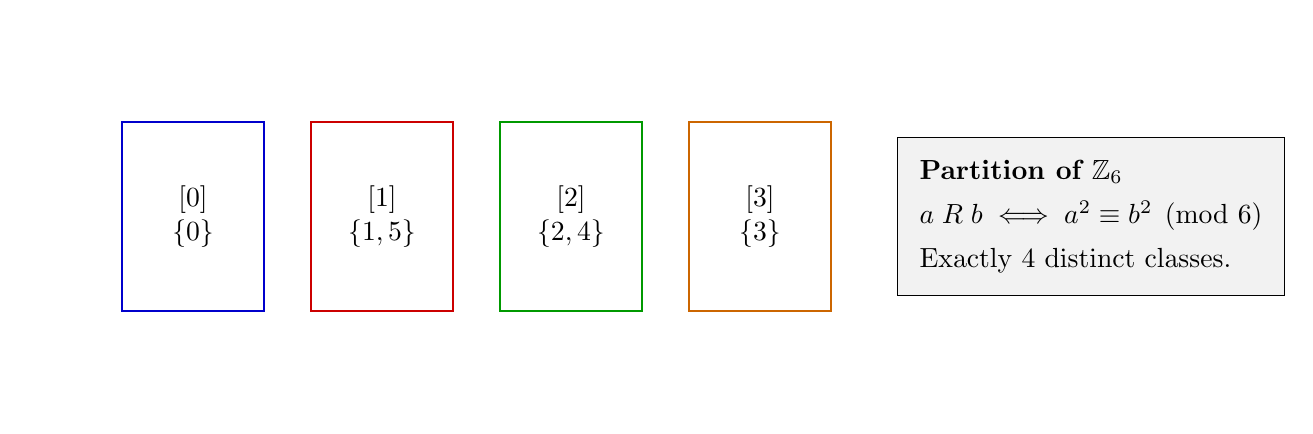
\begin{tikzpicture}[scale=1.2, >=stealth]
        \fill[white] (-1,-1) rectangle (9,3);
        
        \draw[thick, blue!80!black] (0,0) rectangle (1.5,2);
        \node[align=center] at (0.75, 1) {$[0]$\\ $\{0\}$};
        
        \draw[thick, red!80!black] (2,0) rectangle (3.5,2);
        \node[align=center] at (2.75, 1) {$[1]$\\ $\{1, 5\}$};
        
        \draw[thick, green!60!black] (4,0) rectangle (5.5,2);
        \node[align=center] at (4.75, 1) {$[2]$\\ $\{2, 4\}$};
        
        \draw[thick, orange!80!black] (6,0) rectangle (7.5,2);
        \node[align=center] at (6.75, 1) {$[3]$\\ $\{3\}$};
        
        \node[align=left, anchor=west, draw, fill=gray!10, inner sep=8pt] at (8.2, 1) {
            \textbf{Partition of $\Z_6$}\\[4pt]
            $a \mathrel{R} b \iff a^2 \equiv b^2 \pmod{6}$\\[4pt]
            Exactly 4 distinct classes.
        };
    \end{tikzpicture}
    \end{center}

    % Solution 12
    \item \textbf{Solution:}
    We evaluate $x^4 \pmod{5}$ for the standard representatives of $\Z_5$:
    \[ 0^4 = 0 \equiv 0 \pmod{5} \]
    \[ 1^4 = 1 \equiv 1 \pmod{5} \]
    \[ 2^4 = 16 \equiv 1 \pmod{5} \]
    \[ 3^4 = 81 \equiv 1 \pmod{5} \]
    \[ 4^4 = 256 \equiv 1 \pmod{5} \]
    By Fermat's Little Theorem, $x^{p-1} \equiv 1 \pmod{p}$ for all $x \not\equiv 0 \pmod{p}$. Thus, there are only two distinct equivalence classes:
    \begin{align*}
        [0] &= \{x \in \Z \mid x \equiv 0 \pmod{5}\} \\
        [1] &= \{x \in \Z \mid x \not\equiv 0 \pmod{5}\}
    \end{align*}

    % Solution 13
    \item \textbf{Solution:}
    As shown in Problem 3's methodology, $4 \equiv -3 \pmod{7}$. The relation $3a + 4b \equiv 0 \pmod{7}$ becomes $3a - 3b \equiv 0 \pmod{7}$, which is $3(a - b) \equiv 0 \pmod{7}$. Since $\gcd(3, 7) = 1$, this simplifies to $a \equiv b \pmod{7}$. The equivalence classes are simply the standard congruence classes modulo 7:
    \[ [0], [1], [2], [3], [4], [5], [6] \pmod{7} \]

    % Solution 14
    \item \textbf{Solution:}
    For $a^2 + b^2$ to be even, $a^2$ and $b^2$ must have the same parity (both even or both odd). Since $x^2 \equiv x \pmod{2}$ for all integers $x$, $a^2$ and $b^2$ having the same parity implies $a$ and $b$ have the same parity. Thus, $a \mathrel{R} b \iff a \equiv b \pmod{2}$. The distinct equivalence classes are:
    \begin{align*}
        [0] &= \{x \in \Z \mid x \text{ is even}\} \\
        [1] &= \{x \in \Z \mid x \text{ is odd}\}
    \end{align*}

    % Solution 15
    \item \textbf{Solution:}
    The relation is $2a \equiv 2b \pmod{10}$. By definition, this means $10 \mid (2a - 2b)$, which factors to $10 \mid 2(a - b)$. Dividing the divisibility relation by 2 yields $5 \mid (a - b)$, which means $a \equiv b \pmod{5}$. 
    Since the underlying set is $\Z_{10} = \{0, 1, \dots, 9\}$, we group these elements based on their remainder modulo 5:
    \begin{align*}
        [0] &= \{0, 5\} \\
        [1] &= \{1, 6\} \\
        [2] &= \{2, 7\} \\
        [3] &= \{3, 8\} \\
        [4] &= \{4, 9\}
    \end{align*}

    % Solution 16
    \item \textbf{Solution:}
    \begin{proof}
    Assume $a \equiv b \pmod{n}$ and $c \equiv d \pmod{n}$. By definition, there exist integers $k, j$ such that:
    \[ a = b + kn \]
    \[ c = d + jn \]
    Adding these two equations yields:
    \[ a + c = (b + kn) + (d + jn) = (b + d) + n(k + j) \]
    Since $(k + j) \in \Z$, it follows that $n \mid ((a + c) - (b + d))$. Therefore, $a + c \equiv b + d \pmod{n}$.
    \end{proof}

    % Solution 17
    \item \textbf{Solution:}
    \begin{proof}
    We proceed by mathematical induction on $k$.
    \textbf{Base Case ($k=1$):} $a^1 \equiv b^1 \pmod{n}$ is given as true.
    \textbf{Inductive Step:} Assume that for some arbitrary $k \in \N$, $a^k \equiv b^k \pmod{n}$. We must show $a^{k+1} \equiv b^{k+1} \pmod{n}$.
    We know that arithmetic operations (multiplication) are well-defined on equivalence classes. Since $a \equiv b \pmod{n}$ and $a^k \equiv b^k \pmod{n}$, we can multiply the congruences:
    \[ a \cdot a^k \equiv b \cdot b^k \pmod{n} \implies a^{k+1} \equiv b^{k+1} \pmod{n} \]
    By the Principle of Mathematical Induction, the statement holds for all $k \in \N$.
    \end{proof}

    % Solution 18
    \item \textbf{Solution:}
    \begin{proof}
    We test the three properties on $\Z \times (\Z \setminus \{0\})$.
    \begin{itemize}
        \item \textbf{Reflexive:} For any $(a,b)$, $ab = ba$ (commutativity of integers). Thus $(a,b) \mathrel{R} (a,b)$.
        \item \textbf{Symmetric:} Assume $(a,b) \mathrel{R} (c,d)$. Then $ad = bc$. This implies $cb = da$, which means $(c,d) \mathrel{R} (a,b)$.
        \item \textbf{Transitive:} Assume $(a,b) \mathrel{R} (c,d)$ and $(c,d) \mathrel{R} (e,f)$. Then $ad = bc$ and $cf = de$. Multiply the first equation by $f$ to get $adf = bcf$. Substitute $cf = de$ into the right side: $adf = b(de) = bde$. Since $d \neq 0$, we can divide both sides by $d$ to obtain $af = be$. Thus, $(a,b) \mathrel{R} (e,f)$.
    \end{itemize}
    $R$ is an equivalence relation (this formally constructs the rational numbers $\Q$).
    \end{proof}

    % Solution 19
    \item \textbf{Solution:}
    \begin{proof}
    We are given $ac \equiv bc \pmod{n}$, which means $n \mid c(a - b)$. Let $d = \gcd(c,n)$. We can write $n = d n'$ and $c = d c'$, where $\gcd(n', c') = 1$. 
    Substituting these into the divisibility relation gives:
    \[ d n' \mid d c' (a - b) \]
    Dividing by $d$ yields:
    \[ n' \mid c' (a - b) \]
    By Euclid's Lemma, since $n'$ divides the product $c'(a-b)$ and $\gcd(n', c') = 1$, $n'$ must divide $(a - b)$. 
    Thus, $a \equiv b \pmod{n'}$, which is $a \equiv b \pmod{n/d}$.
    \end{proof}

    % Solution 20
    \item \textbf{Solution:}
    \begin{proof}
    Let $R = R_1 \cap R_2$.
    \begin{itemize}
        \item \textbf{Reflexive:} For any $a \in A$, $(a,a) \in R_1$ and $(a,a) \in R_2$ because both are reflexive. Thus, $(a,a) \in R_1 \cap R_2$.
        \item \textbf{Symmetric:} Assume $(a,b) \in R$. Then $(a,b) \in R_1$ and $(a,b) \in R_2$. Because both are symmetric, $(b,a) \in R_1$ and $(b,a) \in R_2$. Thus, $(b,a) \in R$.
        \item \textbf{Transitive:} Assume $(a,b) \in R$ and $(b,c) \in R$. Then $(a,b), (b,c) \in R_1 \implies (a,c) \in R_1$ (since $R_1$ is transitive). Similarly, $(a,c) \in R_2$. Thus, $(a,c) \in R$.
    \end{itemize}
    Therefore, $R_1 \cap R_2$ is an equivalence relation.
    \end{proof}

    % Solution 21
    \item \textbf{Solution:}
    We evaluate $X_{i+1} \equiv (5X_i + 3) \pmod{8}$ starting at $X_0 = 0$:
    \begin{align*}
        X_1 &\equiv 5(0) + 3 \equiv 3 \pmod{8} \\
        X_2 &\equiv 5(3) + 3 = 18 \equiv 2 \pmod{8} \\
        X_3 &\equiv 5(2) + 3 = 13 \equiv 5 \pmod{8} \\
        X_4 &\equiv 5(5) + 3 = 28 \equiv 4 \pmod{8} \\
        X_5 &\equiv 5(4) + 3 = 23 \equiv 7 \pmod{8} \\
        X_6 &\equiv 5(7) + 3 = 38 \equiv 6 \pmod{8} \\
        X_7 &\equiv 5(6) + 3 = 33 \equiv 1 \pmod{8} \\
        X_8 &\equiv 5(1) + 3 = 8 \equiv 0 \pmod{8}
    \end{align*}
    The sequence is $0, 3, 2, 5, 4, 7, 6, 1, 0, \dots$ Yes, it achieves a full period of 8, visiting every equivalence class modulo 8 exactly once before repeating.

    \begin{center}
    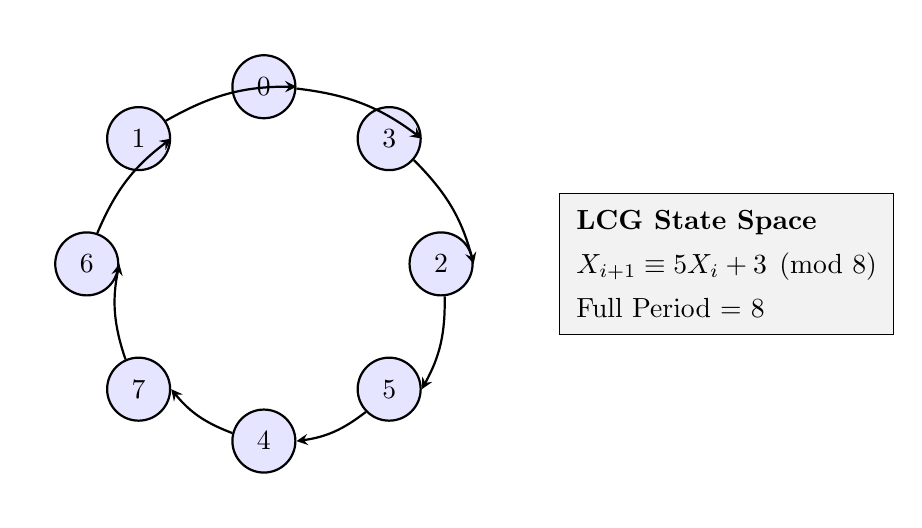
\begin{tikzpicture}[scale=1.5, >=stealth]
        \fill[white] (-2,-2) rectangle (2,2);
        \foreach \i/\label in {0/0, 1/3, 2/2, 3/5, 4/4, 5/7, 6/6, 7/1} {
            \node[circle, draw, thick, fill=blue!10, minimum size=8mm] (N\i) at ({90 - \i*45}:1.5) {\label};
        }
        \foreach \i in {0,...,7} {
            \pgfmathsetmacro{\next}{mod(\i+1,8)}
            \draw[->, thick] (N\i) to[bend left=15] (N\next);
        }
        \node[align=left, anchor=west, draw, fill=gray!10, inner sep=6pt] at (2.5, 0) {
            \textbf{LCG State Space}\\[4pt]
            $X_{i+1} \equiv 5X_i + 3 \pmod{8}$\\[4pt]
            Full Period = 8
        };
    \end{tikzpicture}
    \end{center}

    % Solution 22
    \item \textbf{Solution:}
    We evaluate $h(x) = 2^k \pmod{11}$ for $k \in \{1, 2, 3, 4, 5\}$:
    \begin{align*}
        k=1 &\implies 2^1 = 2 \equiv 2 \pmod{11} \\
        k=2 &\implies 2^2 = 4 \equiv 4 \pmod{11} \\
        k=3 &\implies 2^3 = 8 \equiv 8 \pmod{11} \\
        k=4 &\implies 2^4 = 16 \equiv 5 \pmod{11} \\
        k=5 &\implies 2^5 = 32 \equiv 10 \pmod{11}
    \end{align*}
    The distinct equivalence classes (buckets) populated are $[2], [4], [5], [8], [10] \pmod{11}$.

    % Solution 23
    \item \textbf{Solution:}
    \begin{proof}
    We proceed by induction on $i$.
    \textbf{Base Case ($i=0$):} $X_0 \equiv 0 \pmod{m}$ is given.
    \textbf{Inductive Step:} Assume $X_k \equiv 0 \pmod{m}$ for some arbitrary $k \ge 0$. We evaluate $X_{k+1}$:
    \[ X_{k+1} \equiv a X_k \pmod{m} \]
    Substituting the inductive hypothesis $X_k \equiv 0$:
    \[ X_{k+1} \equiv a(0) = 0 \pmod{m} \]
    By mathematical induction, $X_i \equiv 0 \pmod{m}$ for all $i \ge 0$. The sequence is permanently trapped in $[0]$.
    \end{proof}

    % Solution 24
    \item \textbf{Solution:}
    \begin{proof}
    We must show that $x' \mathrel{R} x$, which means $x' \equiv x \pmod{p}$.
    By definition, $x' = x + kp$ for some integer $k$.
    Subtracting $x$ from both sides yields $x' - x = kp$.
    Since $k \in \Z$, this implies $p \mid (x' - x)$.
    By the definition of congruence, $x' \equiv x \pmod{p}$. Thus, the shifted data point remains in the exact same equivalence class (partition).
    \end{proof}

    % Solution 25
    \item \textbf{Solution:}
    \begin{proof}
    The LCG is $X_{i+1} \equiv X_i + c \pmod{m}$. By expanding this recursively, we find the closed-form state equation:
    \[ X_k \equiv X_0 + kc \pmod{m} \]
    For the generator to have a full period of $m$, it must visit $m$ distinct states before repeating. It repeats when $X_k \equiv X_0 \pmod{m}$ for $k > 0$.
    \[ X_0 + kc \equiv X_0 \pmod{m} \implies kc \equiv 0 \pmod{m} \implies m \mid kc \]
    The period is the smallest positive integer $k$ such that $m \mid kc$. 
    If $\gcd(c,m) = 1$, by Euclid's Lemma, $m \mid k$, so the smallest such $k$ is $m$. Thus, it has full period.
    If $\gcd(c,m) = d > 1$, then let $k = m/d$. Since $d > 1$, $k < m$. Then $kc = (m/d)c = m(c/d)$. Since $d \mid c$, $(c/d)$ is an integer, so $m \mid kc$. The sequence repeats at $k < m$, failing to achieve full period.
    Thus, full period $m \iff \gcd(c,m) = 1$.
    \end{proof}

    % Solution 26
    \item \textbf{Solution:}
    \textbf{Flaw:} The proof commits the \textit{Exponentiation Fallacy}. Modular arithmetic allows substitution in the base, but \textbf{not} in the exponent. Exponents operate in a different algebraic structure (specifically, they must be evaluated modulo $\phi(n)$ via Euler's Totient Theorem, not modulo $n$).\\
    \textbf{Counterexample:} Let $a = 1$ and $b = 6$. Clearly, $1 \equiv 6 \pmod{5}$. However, evaluating the powers yields $2^1 = 2$ and $2^6 = 64$. Modulo 5, $64 \equiv 4 \pmod{5}$. Since $2 \not\equiv 4 \pmod{5}$, the claim is false.

    % Solution 27
    \item \textbf{Solution:}
    \textbf{Flaw:} The logical flaw occurs in the deduction regarding parity. The proof correctly states that $(a+b) + (b+c) = a + 2b + c$. However, it falsely claims that because $a+b$ is odd and $b+c$ is odd, their sum is odd. The sum of two odd numbers is \textbf{even}. Therefore, $a + 2b + c$ is even. Since $2b$ is even, $a+c$ must be \textbf{even}. The relation requires $a+c$ to be odd for $a \mathrel{R} c$ to hold. Because $a+c$ is even, $a \not\mathrel{R} c$, meaning transitivity actually \textbf{fails}.

    % Solution 28
    \item \textbf{Solution:}
    \textbf{Flaw:} The proof commits the \textit{Cancellation Fallacy}. When dividing a divisibility relation $6 \mid 2(x-y)$ by a constant $c=2$, you must also divide the modulus by $\gcd(c, n)$. Here, $\gcd(2, 6) = 2 \neq 1$. The correct deduction is $(6/2) \mid (x-y)$, which means $3 \mid (x-y)$, leading to $x \equiv y \pmod{3}$, not modulo 6. \\
    \textbf{Counterexample:} Let $x = 4$ and $y = 1$. $2(4) = 8 \equiv 2 \pmod{6}$ and $2(1) = 2 \equiv 2 \pmod{6}$. Thus $2x \equiv 2y \pmod{6}$ holds. But $4 \not\equiv 1 \pmod{6}$.

    % Solution 29
    \item \textbf{Solution:}
    \textbf{Flaw:} The proof fundamentally misunderstands the definition of the Symmetric property. Symmetry requires that if $a \mathrel{R} b$, then $b \mathrel{R} a$. In the context of this relation, $b \mathrel{R} a$ strictly means $b \le a$. The proof deduces $b \ge a$, which is algebraically correct but represents the \textit{opposite} relation, not $b \mathrel{R} a$. \\
    \textbf{Counterexample:} $2 \le 3$ is true ($2 \mathrel{R} 3$), but $3 \le 2$ is false ($3 \not\mathrel{R} 2$). The relation is anti-symmetric, not symmetric.

    % Solution 30
    \item \textbf{Solution:}
    \textbf{Flaw:} The proof falsely invokes Euclid's Lemma without the prerequisite that $n$ is prime. If $n$ is composite, it can divide a product $(a-b)(a+b)$ by having its prime factors split between the two terms, without dividing either term entirely.\\
    \textbf{Counterexample:} Let $n = 8$, $a = 3$, $b = 1$. $3^2 = 9 \equiv 1 \pmod{8}$ and $1^2 = 1 \equiv 1 \pmod{8}$. Thus $a^2 \equiv b^2 \pmod{8}$. However, $3 \not\equiv 1 \pmod{8}$ and $3 \not\equiv -1 \pmod{8}$ (since $-1 \equiv 7 \pmod{8}$). The claim fails for composite moduli.

\end{enumerate}

\newpage

\section{Concept Checklist \& Question Mapping (Reference)}

\renewcommand{\arraystretch}{1.5}
\noindent
\begin{tabularx}{\textwidth}{l X l}
\toprule
\textbf{ID} & \textbf{Concept / Technique} & \textbf{Problem Mapping} \\
\midrule
C1 & Direct Verification of Equivalence Relations (Linear Combinations) & 1, 3, 13 \\
C2 & Direct Verification of Equivalence Relations (Non-linear/Polynomial) & 2, 5, 11, 12 \\
C3 & Counterexample Generation (Failing Reflexivity) & 6 \\
C4 & Counterexample Generation (Failing Symmetry/Transitivity) & 7, 8, 10 \\
C5 & Equivalence Class Determination (Exhaustive Evaluation) & 11, 12, 13, 14, 15 \\
C6 & The ``Add and Subtract'' Trick \& Modular Substitution & 1, 2, 3 \\
C7 & Modular Cancellation and GCD Conditions & 3, 15, 19 \\
C8 & Well-definedness of Arithmetic Operations on Quotient Spaces & 16, 17 \\
C9 & Real-World Modeling: Linear Congruential Generators (LCGs) & 21, 23, 25 \\
C10 & Real-World Modeling: Hashing and Partitions & 22, 24 \\
C11 & Diagnostic Testing: Identifying Logical Flaws (Cancellation Fallacy) & 9, 28, 30 \\
C12 & Diagnostic Testing: Identifying Logical Flaws (Exponentiation Fallacy) & 26 \\
C13 & Diagnostic Testing: Identifying Logical Flaws (Vacuous Truths \& Logic) & 27, 29 \\
C14 & Abstract Extensions (Relations on $\R$, $\R^2$, or Cartesian Products) & 4, 18, 20 \\
\bottomrule
\end{tabularx}

\end{document}